Considering the estimation methodology in \hyperref[appendix:sigma]{appendix C}, I obtain a capital-labor elasticity of substitution around 1.279 for France over the period 1970-2010. However, the estimated coefficient is only significant at a 90\% confidence level. Such a result may be due to a break in the regime of $\sigma$. The relationship between the labor-to-capital income ratio $\Theta_t$ and the capital-per-worker $k_t$ depends on the value of $\sigma$ with respect to unity. From the comparatives statics derived in section \ref{sec:model}, it can be shown that :
\begin{equation*}
	\frac{\partial \Theta_t}{\partial k_t} \gtreqqless 0 ~~ \text{when} ~~ \sigma \lesseqqgtr 1
\end{equation*}
When both input factors are gross complement (i.e. $\sigma < 1$), the labor-to-capital income ratio and the capital-per-worker vary in the same direction. While they vary in opposite ways under gross substituability. The elasticity of substitution $\sigma$ is estimated using the following equation :
\begin{equation*}
\ln \Theta_t = \alpha + \frac{1-\sigma}{\sigma} \ln \tilde{k}_t + \frac{1-\sigma}{\sigma}(a_K-a_L)\left(t-t_0\right)
\end{equation*}
Inspecting the time series of $\ln \Theta_t$ and $\ln \tilde{k}_t$, I suspect that there is a change of regime in the link between them. Figure \ref{fig:k_Theta_log} plots these time series.
\begin{figure}[tb]
	\centering
	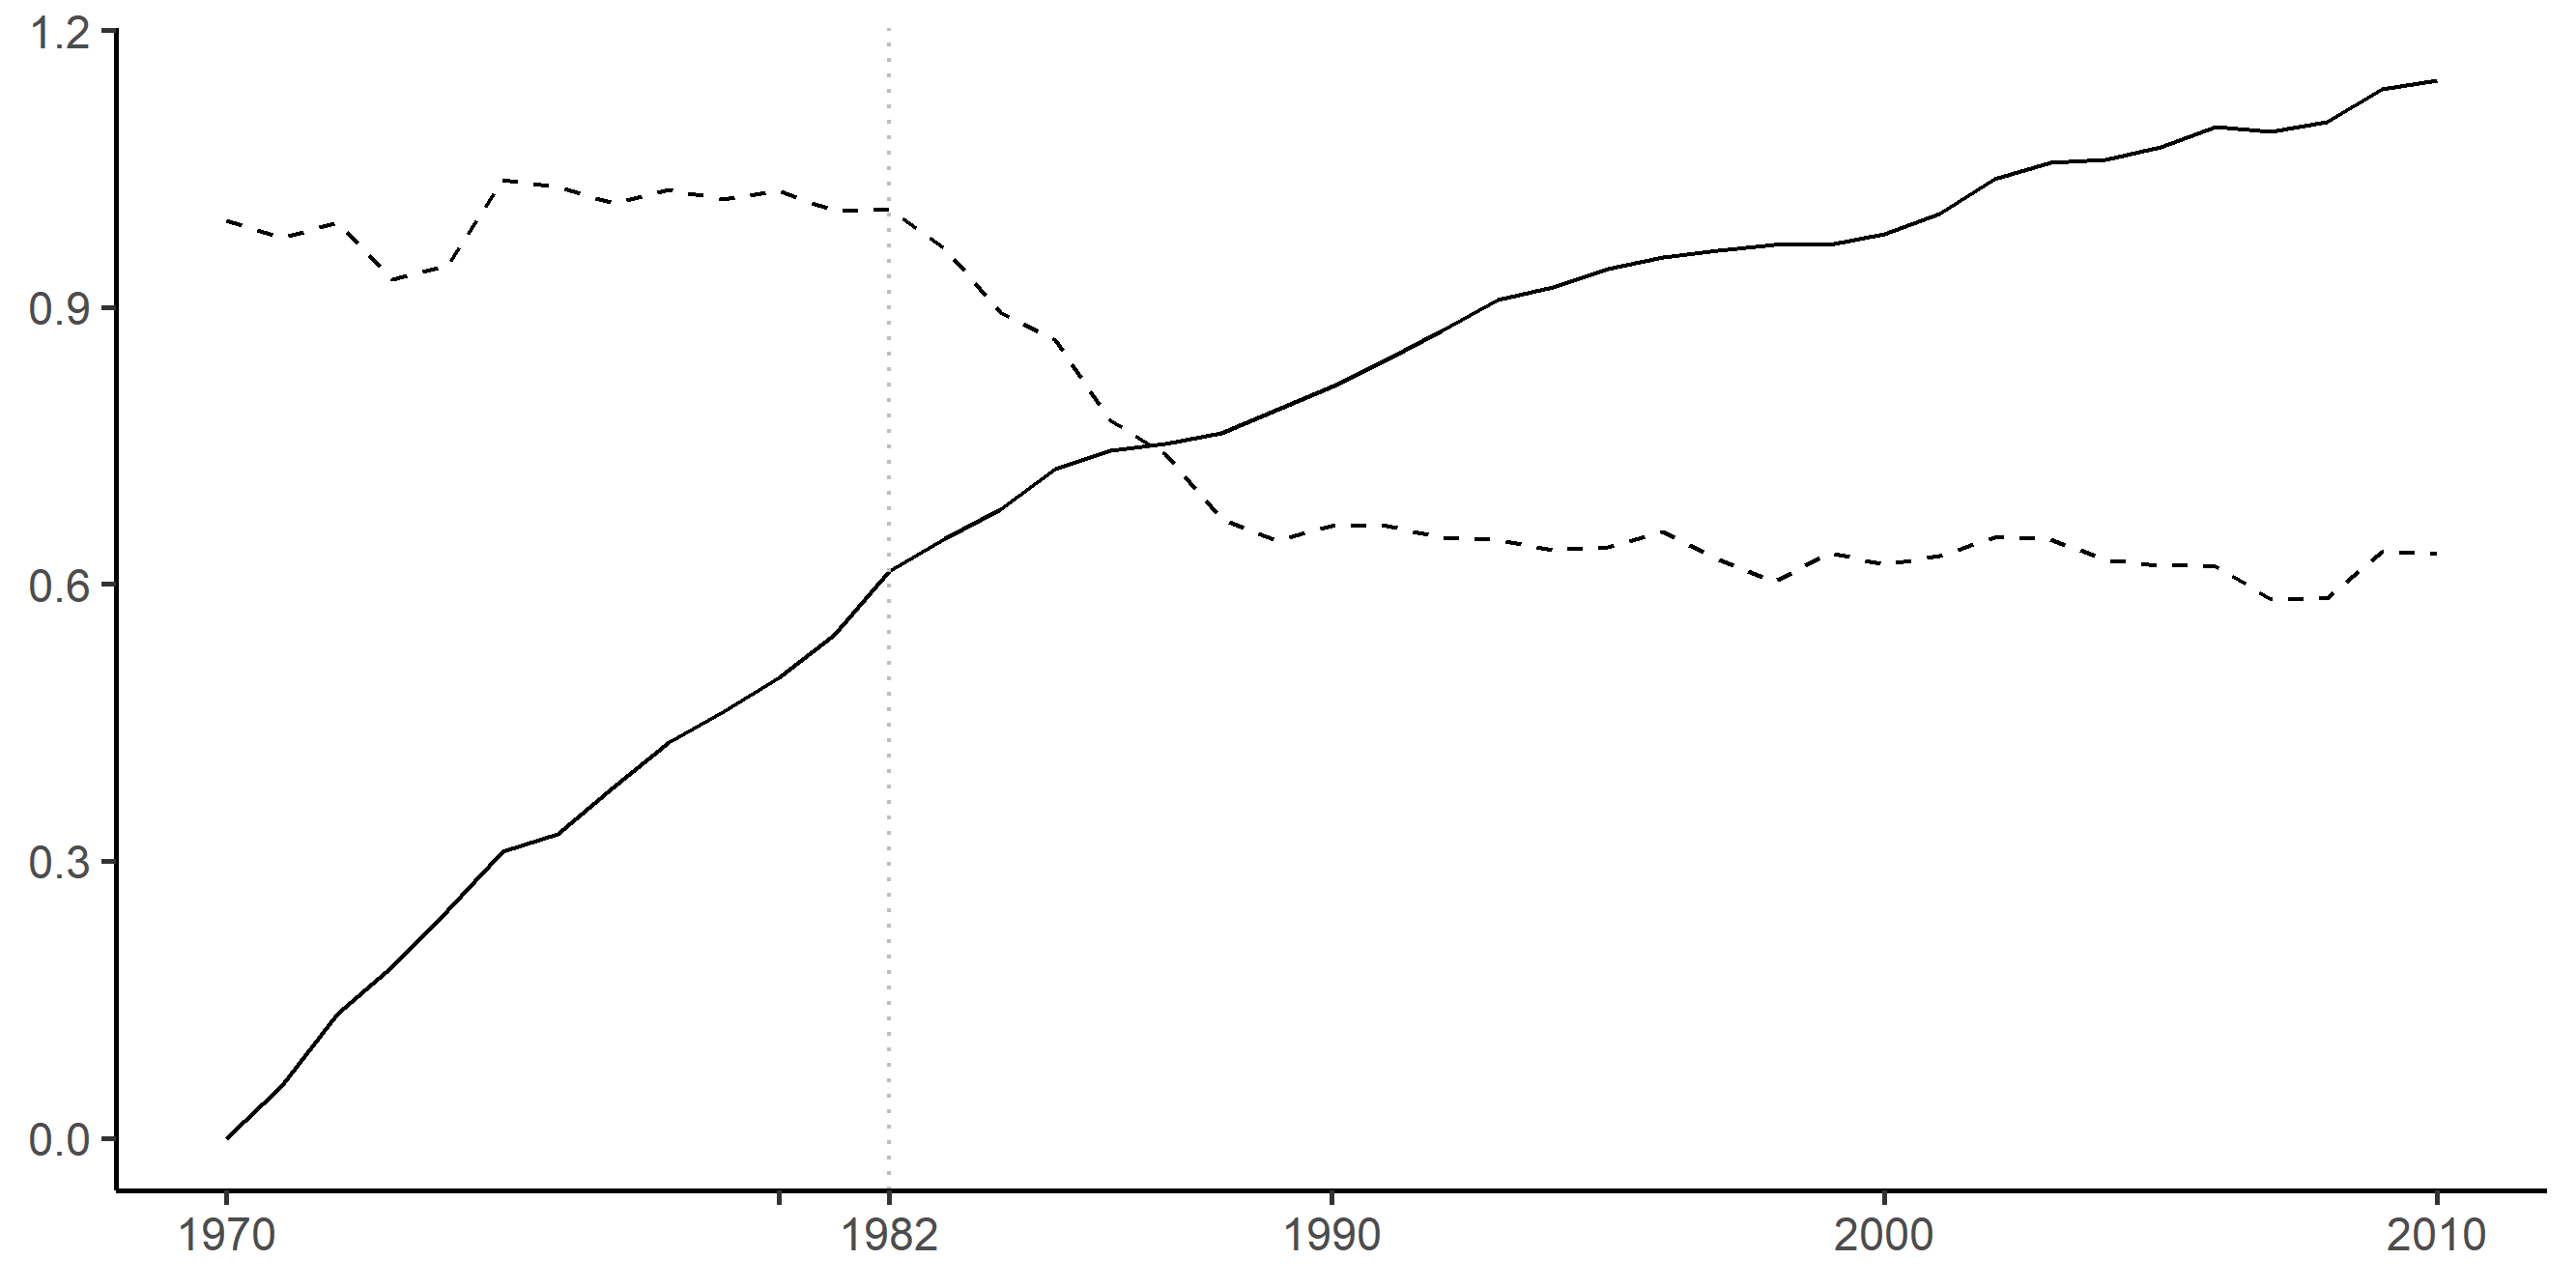
\includegraphics[width=1\linewidth]{../result/appendix_CD/k_Theta_log.png}
	\caption{$\ln \tilde{k}_t$ (red) and $\ln \Theta_t$ (blue) for France over the period 1970-2010.}
	\label{fig:k_Theta_log}
\end{figure}
The figure suggests that the correlation between both variables is different before and after the beginning of the 80's. Suppose that the change of regime in the relationship has occurred in 1982. The correlation between both variables is about 0.305 before 1982 and -0.787 after.\footnote{The year 1982 is included in the first sub-sample. Including it in the sub-sample after the break leads to the correlations of 0.499 and -0.786 for before and after respectively.} Such a difference in the correlation suggests that there are two regimes. However, the biased technical change has not been considered so far. Therefore, I have to detrend both variables in order to check whether the regime change is not driven by it. Using the Frisch-Waugh-Lovell theorem, I regress each variable on a linear time trend and extract the residuals as detrended variables. Both regressions correspond to the following:
\begin{align*}
	\ln \Theta_t &= \varphi_0^\Theta + \varphi_1^\Theta \times t + \varepsilon_t^\Theta \\
	\ln \tilde{k}_t &= \varphi_0^{\tilde{k}} + \varphi_1^{\tilde{k}} \times t + \varepsilon_t^{\tilde{k}}
\end{align*}
Figure \ref{fig:k_Theta_log_detrend} displays both detrended variables $\varepsilon_t^{\tilde{k}}$ and $\varepsilon_t^\Theta$. The vertical dashed lines correspond to potential break years in the regime. Looking at the variables behavior before and after the three thresholds, it suggests that there are still two regimes. Therefore, this result remains even when controlling for linear biased technical change.
\begin{figure}[tb]
	\centering
	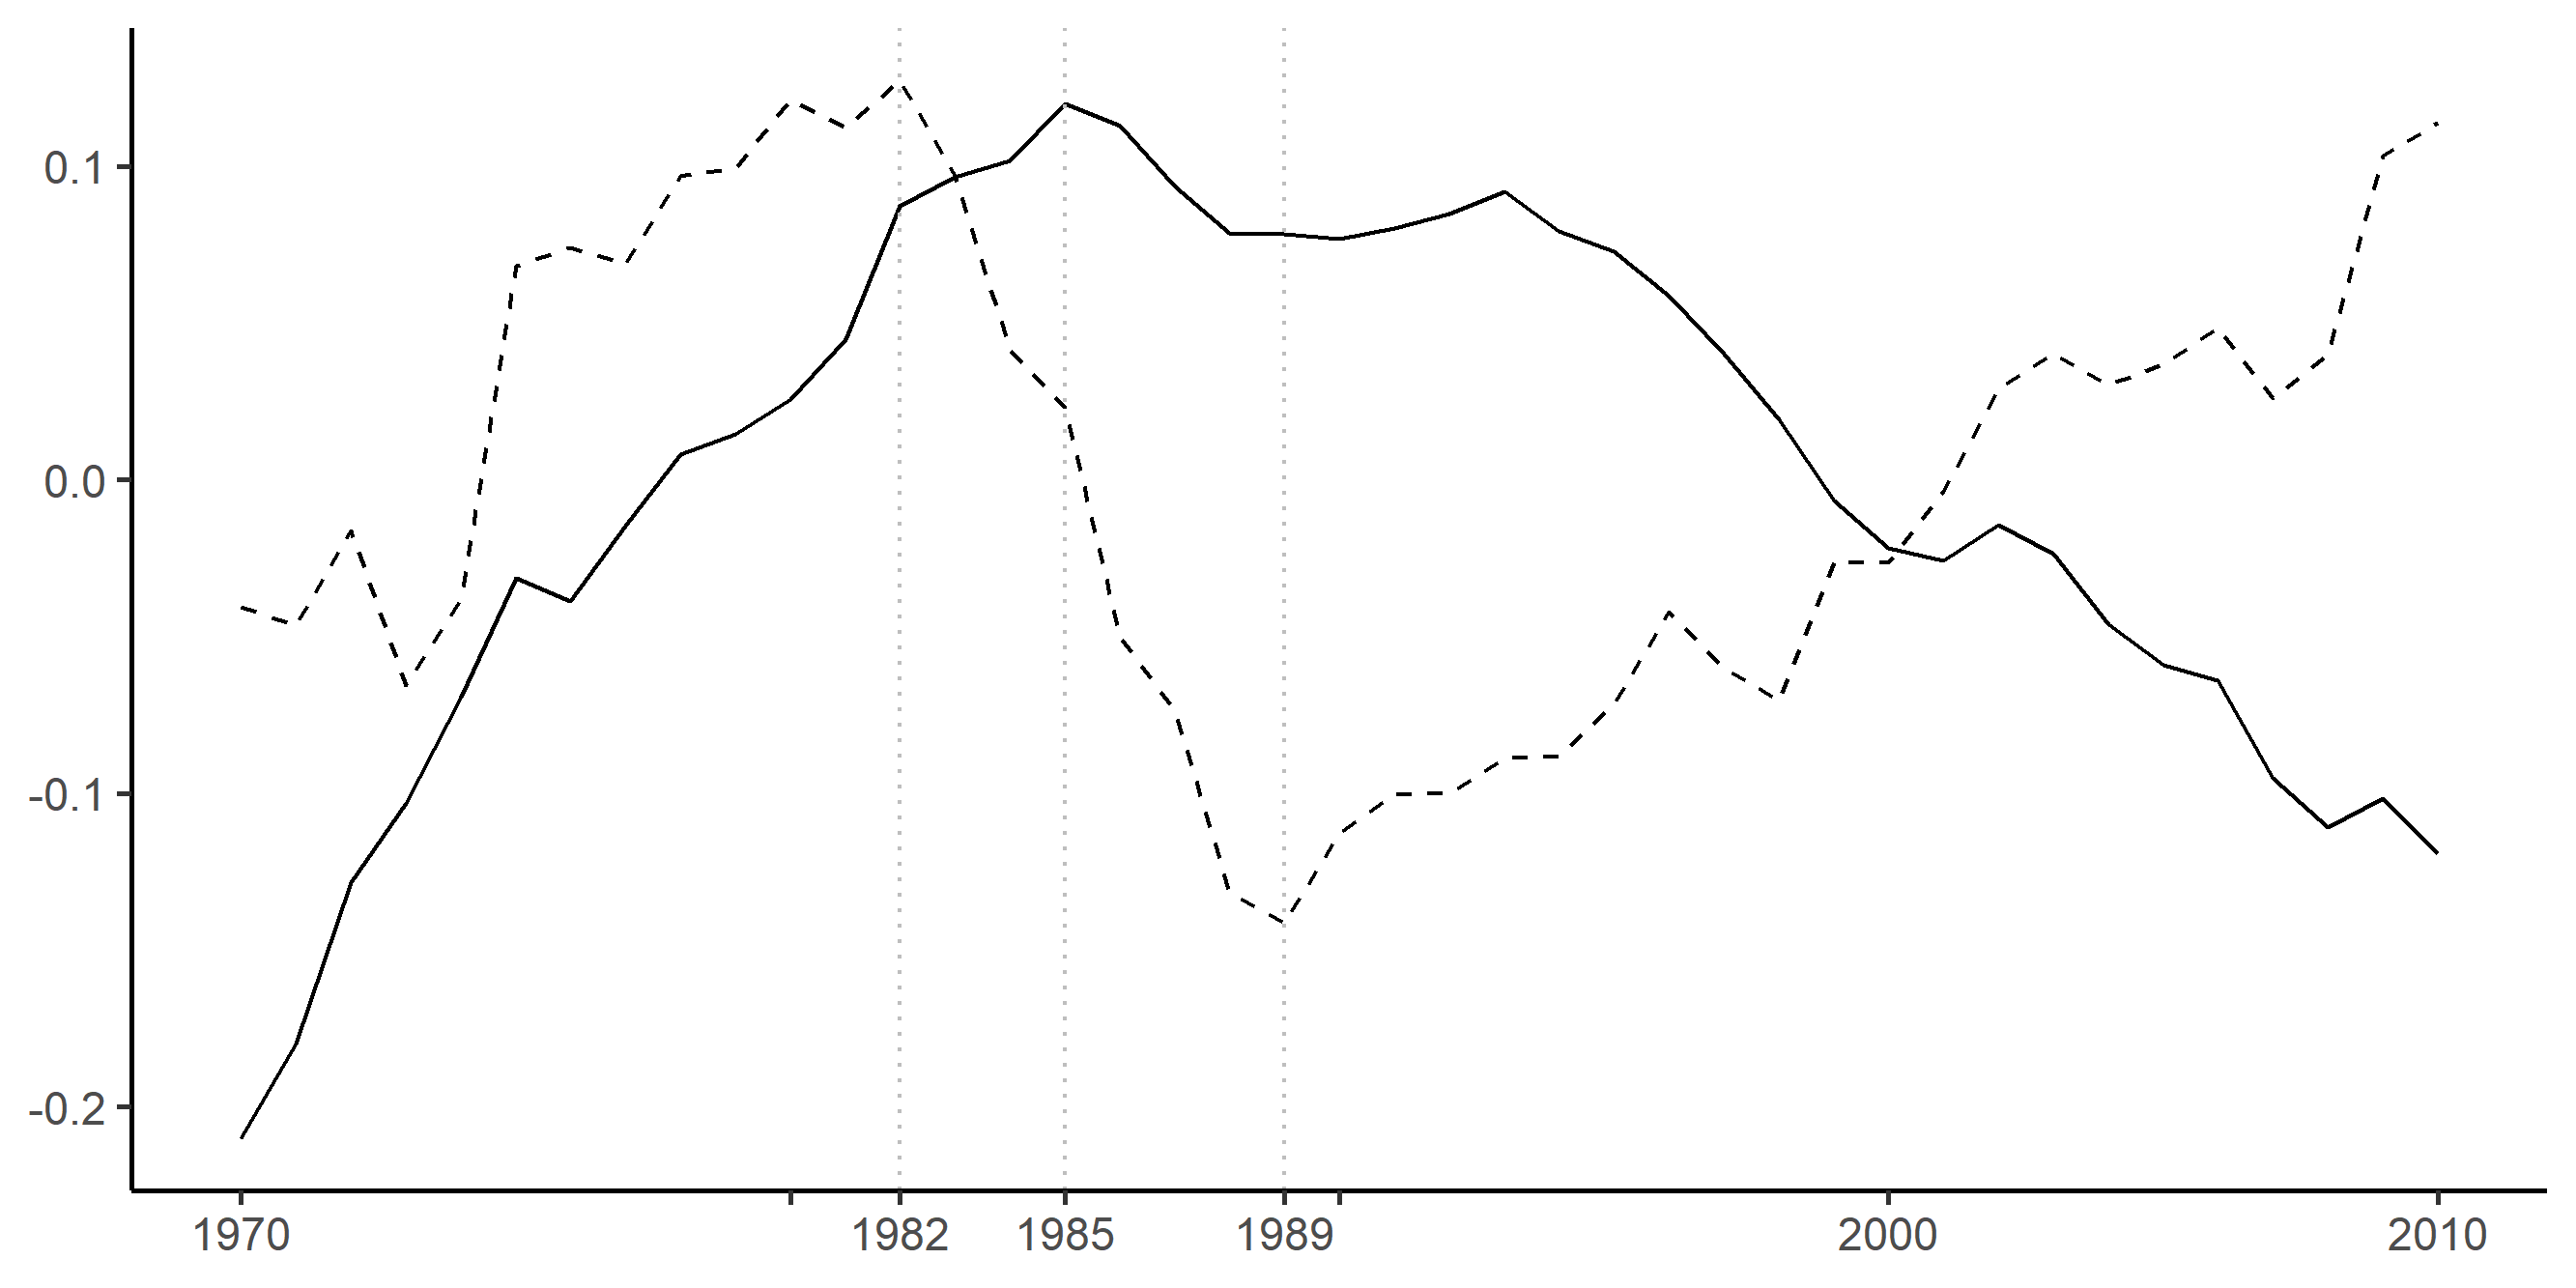
\includegraphics[width=1\linewidth]{../result/appendix_CD/k_Theta_log_detrend.png}
	\caption{$\varepsilon_t^{\tilde{k}}$ (red) and $\varepsilon_t^\Theta$ (blue) for France over the period 1970-2010.}
	\label{fig:k_Theta_log_detrend}
\end{figure}

For instance, figure \ref{fig:k_Theta_log_reg85} plots the regression lines before and after an elasticity regime change in 1985. The slope is positive between 1970 and 1985, so the elasticity would be smaller than 1 during this period and greater thereafter. All years between 1980 and 1990 are candidate to be the break year.
\begin{figure}[tb]
	\centering
	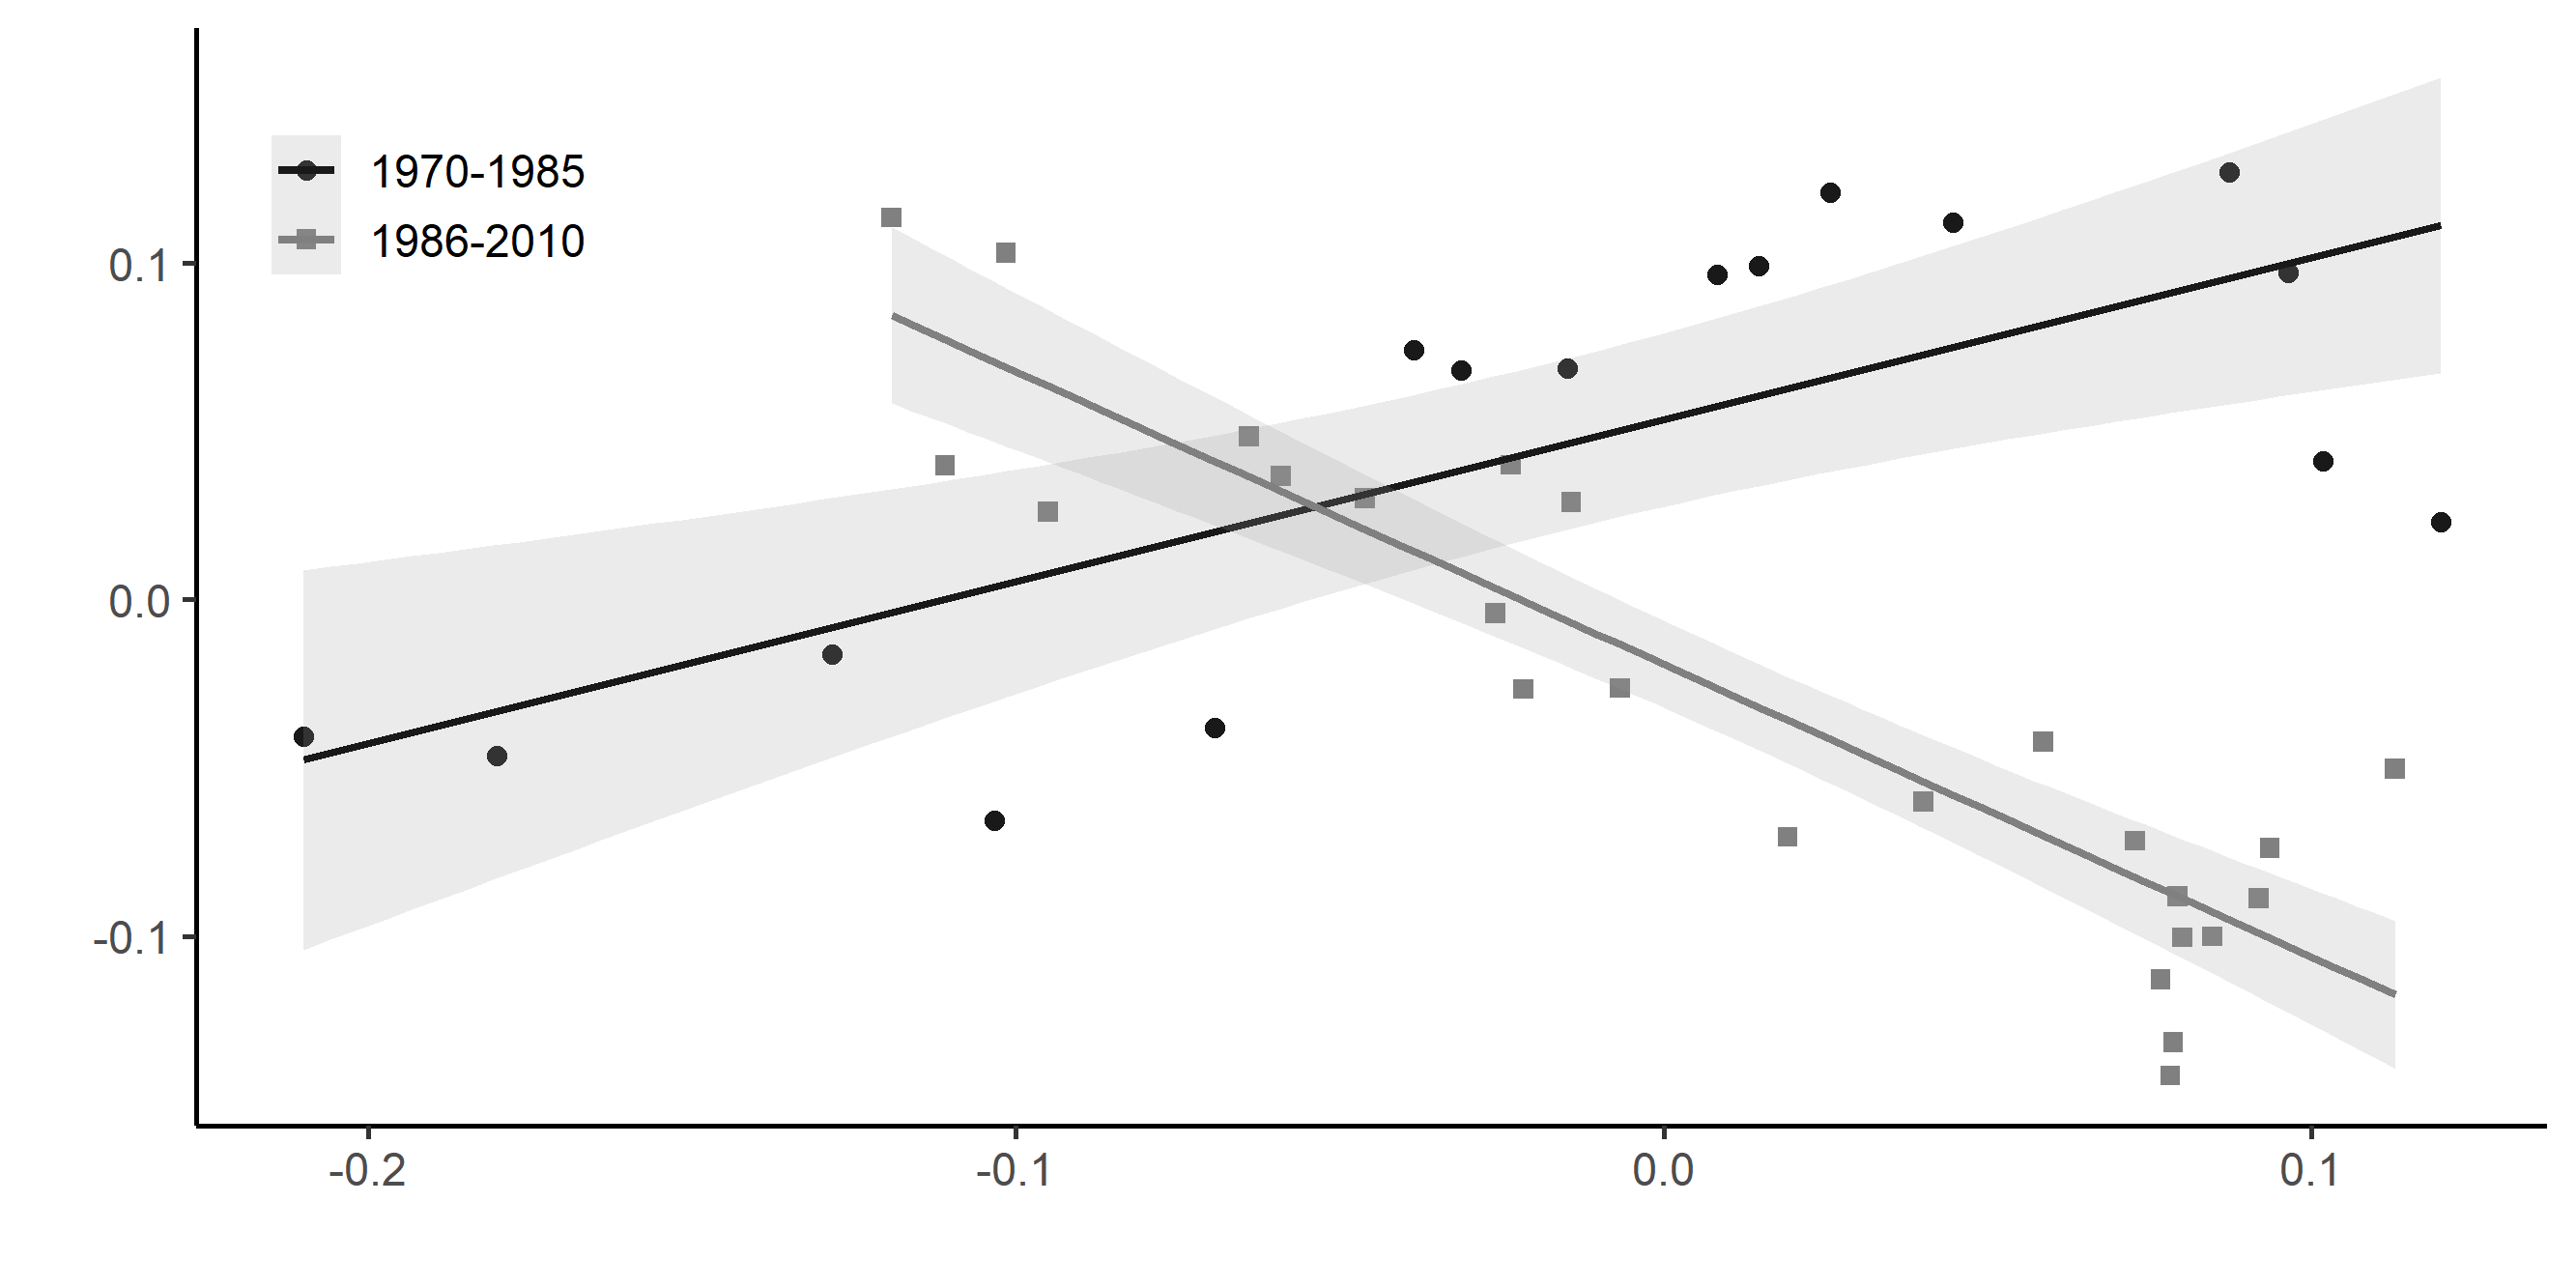
\includegraphics[width=1\linewidth]{../result/appendix_CD/k_Theta_log_reg85.png}
	\caption{Relationship between $\varepsilon_t^{\tilde{k}}$ (x-axis) and $\varepsilon_t^\Theta$ (y-axis) for France over the period 1970-2010.}
	\label{fig:k_Theta_log_reg85}
	\vspace{.5ex}
	\hrule
	\vspace{-4ex}
	\justify\singlespacing\footnotesize The gray area corresponds to the confidence interval of the associated regression. The level of the confidence interval is set to 0.95.
\end{figure}

To find which year corresponds to the most efficient break year, I run multiple regressions by changing the break year $\bar{t}$ for each regression. The estimated equation is:
\begin{equation*}
	\varepsilon_t^{\Theta} = \nu_1 \mathds{1}_{\lbrace t \leq \bar{t} \rbrace} + \nu_2 \mathds{1}_{\lbrace t > \bar{t} \rbrace} + \rho_1 \mathds{1}_{\lbrace t \leq \bar{t} \rbrace} \varepsilon_t^{\tilde{k}} + \rho_2 \mathds{1}_{\lbrace t > \bar{t} \rbrace} \varepsilon_t^{\tilde{k}} + \zeta_t
\end{equation*}
where $\mathds{1}$ is a dummy variable which is equal to 1 when the condition under brackets is satisfied, 0 otherwise. Table \ref{tab:break} displays the four coefficients (i.e. $\nu_1$, $\nu_2$, $\rho_1$, $\rho_2$) and the $R^2$ of each regression. The regression with a change in the regime in 1985 (i.e. $\bar{t} = 1985$) has the greatest $R^2$ and all its coefficients are significant. Thus, I assume that the break in the regime has occurred in 1985.
% Table break
\begingroup
\renewcommand{\arraystretch}{1}
\begin{table}[tb]
	\caption{Estimation of the capital-labor elasticity of substitution for France with break year}\label{tab:break}
	\centering
	\begin{threeparttable}
		\begin{tabular}{c D{.}{.}{-3} D{.}{.}{-3} D{.}{.}{-3} D{.}{.}{-3} D{.}{.}{-3}}
			$\bar{t}$ 	& \multicolumn{1}{c}{$\nu_1$} & \multicolumn{1}{c}{$\nu_2$} & \multicolumn{1}{c}{$\rho_1$} & \multicolumn{1}{c}{$\rho_2$} & \multicolumn{1}{c}{$R^2$} \\ \hline \hline \\ [-1ex]
	%		1974		& -0.044 		& 0.017 		& -0.017 		& -0.564^{***} 	& 0.264 \\
	%					& (0.090)		& (0.012)		& (0.610)		& (0.168)		& \\
	%		1975		& 0.028			& 0.015			& 0.424			& -0.554^{***}	& 0.244 \\
	%					& (0.090)		& (0.012)		& (0.610)		& (0.168)		& \\
	%		1976		& 0.054			& 0.014			& 0.580			& -0.540^{***}	& 0.239 \\
	%					& (0.053)		& (0.013)		& (0.421)		& (0.174)		& \\
	%		1977		& 0.062			& 0.012			& 0.634^{*}		& -0.529^{***}	& 0.247 \\
	%					& (0.044)		& (0.013)		& (0.371)		& (0.174)		& \\
	%		1978		& 0.070^{*}		& 0.009			& 0.694^{**}	& -0.520^{***}	& 0.278 \\
	%					& (0.036)		& (0.013)		& (0.322)		& (0.171)		& \\
	%		1979		& 0.075^{**}	& 0.006			& 0.725^{**}	& -0.514^{***}	& 0.317 \\
	%					& (0.030)		& (0.013)		& (0.286)		& (0.166)		& \\
			1980		& 0.080^{***}	& 0.002			& 0.765^{***}	& -0.516^{***}	& 0.385 \\
						& (0.025)		& (0.012)		& (0.251)		& (0.158)		& \\
			1981		& 0.079^{***}	& -0.002		& 0.762^{***}	& -0.533^{***}	& 0.461 \\
						& (0.021)		& (0.012)		& (0.217)		& (0.148)		& \\
			1982		& 0.077^{***}	& -0.007		& 0.736^{***}	& -0.607^{***}	& 0.596 \\
						& (0.016)		& (0.010)		& (0.168)		& (0.130)		& \\
			1983		& 0.071^{***}	& -0.012		& 0.677^{***}	& -0.690^{***}	& 0.705 \\
						& (0.013)		& (0.009)		& (0.131)		& (0.113)		& \\
			1984		& 0.062^{***}	& -0.015^{*}	& 0.580^{***}	& -0.764^{***}	& 0.741 \\
						& (0.011)		& (0.008)		& (0.114)		& (0.108)		& \\
			1985		& 0.053^{***}	& -0.019^{**}	& 0.482^{***}	& -0.870^{***}	& 0.780 \\
						& (0.010)		& (0.008)		& (0.098)		& (0.104)		& \\
			1986		& 0.043^{***}	& -0.022^{**}	& 0.365^{***}	& -0.928^{***}	& 0.713 \\
						& (0.011)		& (0.009)		& (0.106)		& (0.124)		& \\
			1987		& 0.034^{***}	& -0.023^{**}	& 0.282^{**}	& -0.956^{***}	& 0.635 \\
						& (0.012)		& (0.010)		& (0.116)		& (0.145)		& \\
			1988		& 0.024^{*}		& -0.022^{*}	& 0.202			& -0.931^{***}	& 0.507 \\
						& (0.013)		& (0.012)		& (0.133)		& (0.173)		& \\
			1989		& 0.016			& -0.019		& 0.131			& -0.893^{***}	& 0.391 \\
						& (0.014)		& (0.014)		& (0.145)		& (0.198)		& \\
			1990		& 0.009			& -0.018		& 0.082			& -0.871^{***}	& 0.321 \\
						& (0.015)		& (0.015)		& (0.151)		& (0.216)		& \\
			\hline \hline
		\end{tabular}
		\begin{tablenotes}
		{\footnotesize 
			\item \textit{Note :} $^{*}$p$<$0.1; $^{**}$p$<$0.05; $^{***}$p$<$0.01. Standard errors in parentheses.
		}
		\end{tablenotes}
	\end{threeparttable}
\end{table}
\endgroup
I have to estimate a value of $\sigma$ for 1970-1985 and another one for 1986-2010. I estimate the equation \eqref{eq:est_sigma} for each sub-sample with and without biased technical change. Table \ref{tab:sigma_sub} summarizes the results. 
% Table sigma
	\begingroup
\renewcommand{\arraystretch}{1}
\begin{table}[tb]
	\caption{Estimation of the capital-labor elasticity of substitution ($\sigma$) for France with break in the regime in 1986.}\label{tab:sigma_sub}
	\centering
	\begin{threeparttable}
		\begin{tabular}{c D{.}{.}{-3} D{.}{.}{-3} D{.}{.}{-3} D{.}{.}{-3}}
			Sample & \multicolumn{2}{c}{1970-1985} & \multicolumn{2}{c}{1986-2010} \\ \hline \hline \\ [-1ex]
			$\alpha$ 							& 1.007^{***} 	& 0.970^{***}	& 0.877^{***}	& 0.916^{***}	\\
												& (0.026)		& (0.040)		& (0.046)		& (0.160)		\\
			$\frac{1-\sigma}{\sigma}$ 			& -0.062	 	& 1.002			& -0.243^{***}	& -0.322 		\\
												& (0.059)		& (0.648)		& (0.048)		& (0.321)			\\
			$\frac{1-\sigma}{\sigma}(a_K-a_L)$ 	& 				& -0.050		&				& 0.001	\\
												& 				& (0.031)		& 				& (0.005)		\\ [1ex] \hline \\ [-1ex]
			Hours worked correction 			& \multicolumn{1}{c}{Yes} 	& \multicolumn{1}{c}{Yes} & \multicolumn{1}{c}{Yes} & \multicolumn{1}{c}{Yes} \\
			Biased technical change 			& \multicolumn{1}{c}{No} 	& \multicolumn{1}{c}{Yes} & \multicolumn{1}{c}{No} & \multicolumn{1}{c}{Yes} \\ [1ex] \hline \\ [-1ex]		
			$\sigma$ 							& 1.067			& 0.499			& 1.321			& 1.476		\\ [1ex]
			\hline \hline
		\end{tabular}
		\begin{tablenotes}
		{\footnotesize 
			\item \textit{Note :} $^{*}$p$<$0.1; $^{**}$p$<$0.05; $^{***}$p$<$0.01. Standard errors in parentheses.
		}
		\end{tablenotes}
	\end{threeparttable}
\end{table}
\endgroup
Biased technical change coefficients are not significant in both sub-sample regressions, neither are the coefficients associated to the elasticity. Therefore, I take into account the estimate where the technical change is not biased. Between 1970 and 1985, I set the capital-labor elasticity of substitution to unity, since the coefficient is not statistically different from 0.\footnote{This is mainly due to the lack of observations. The sub-sample has only 16 observations and therefore 14 degrees of freedom.} However, it is significant between 1986 and 2010 and the elasticity is about 1.321.